\documentclass[tikz]{standalone}
\usetikzlibrary{shapes}
\tikzset{
    recyel/.style={draw,minimum width=3cm,minimum height=2cm,align=center,text width=3cm,fill=yellow!50,font=\sffamily},
    rndred/.style={rounded corners=1cm,draw,minimum width=3cm,minimum height=2cm,align=center,text width=3cm,fill=red!30,font=\sffamily},
    rndyel/.style={rounded corners=1cm,draw,minimum width=3cm,minimum height=2cm,align=center,text width=3cm,fill=yellow!50,font=\sffamily},
    diared/.style={diamond,draw,minimum width=3cm,minimum height=2cm,align=center,text width=3cm,fill=red!50,font=\sffamily,aspect=1.5},
    diayel/.style={diamond,draw,minimum width=3cm,minimum height=2cm,align=center,text width=3cm,fill=yellow!50,font=\sffamily,aspect=1.5},
    cylwht/.style={cylinder,draw,shape aspect=.5,cylinder uses custom fill,cylinder end fill=white,minimum width=1cm,minimum height=1cm,cylinder body fill=white,opacity=1,scale=2,rotate=90}
}
\begin{document}
    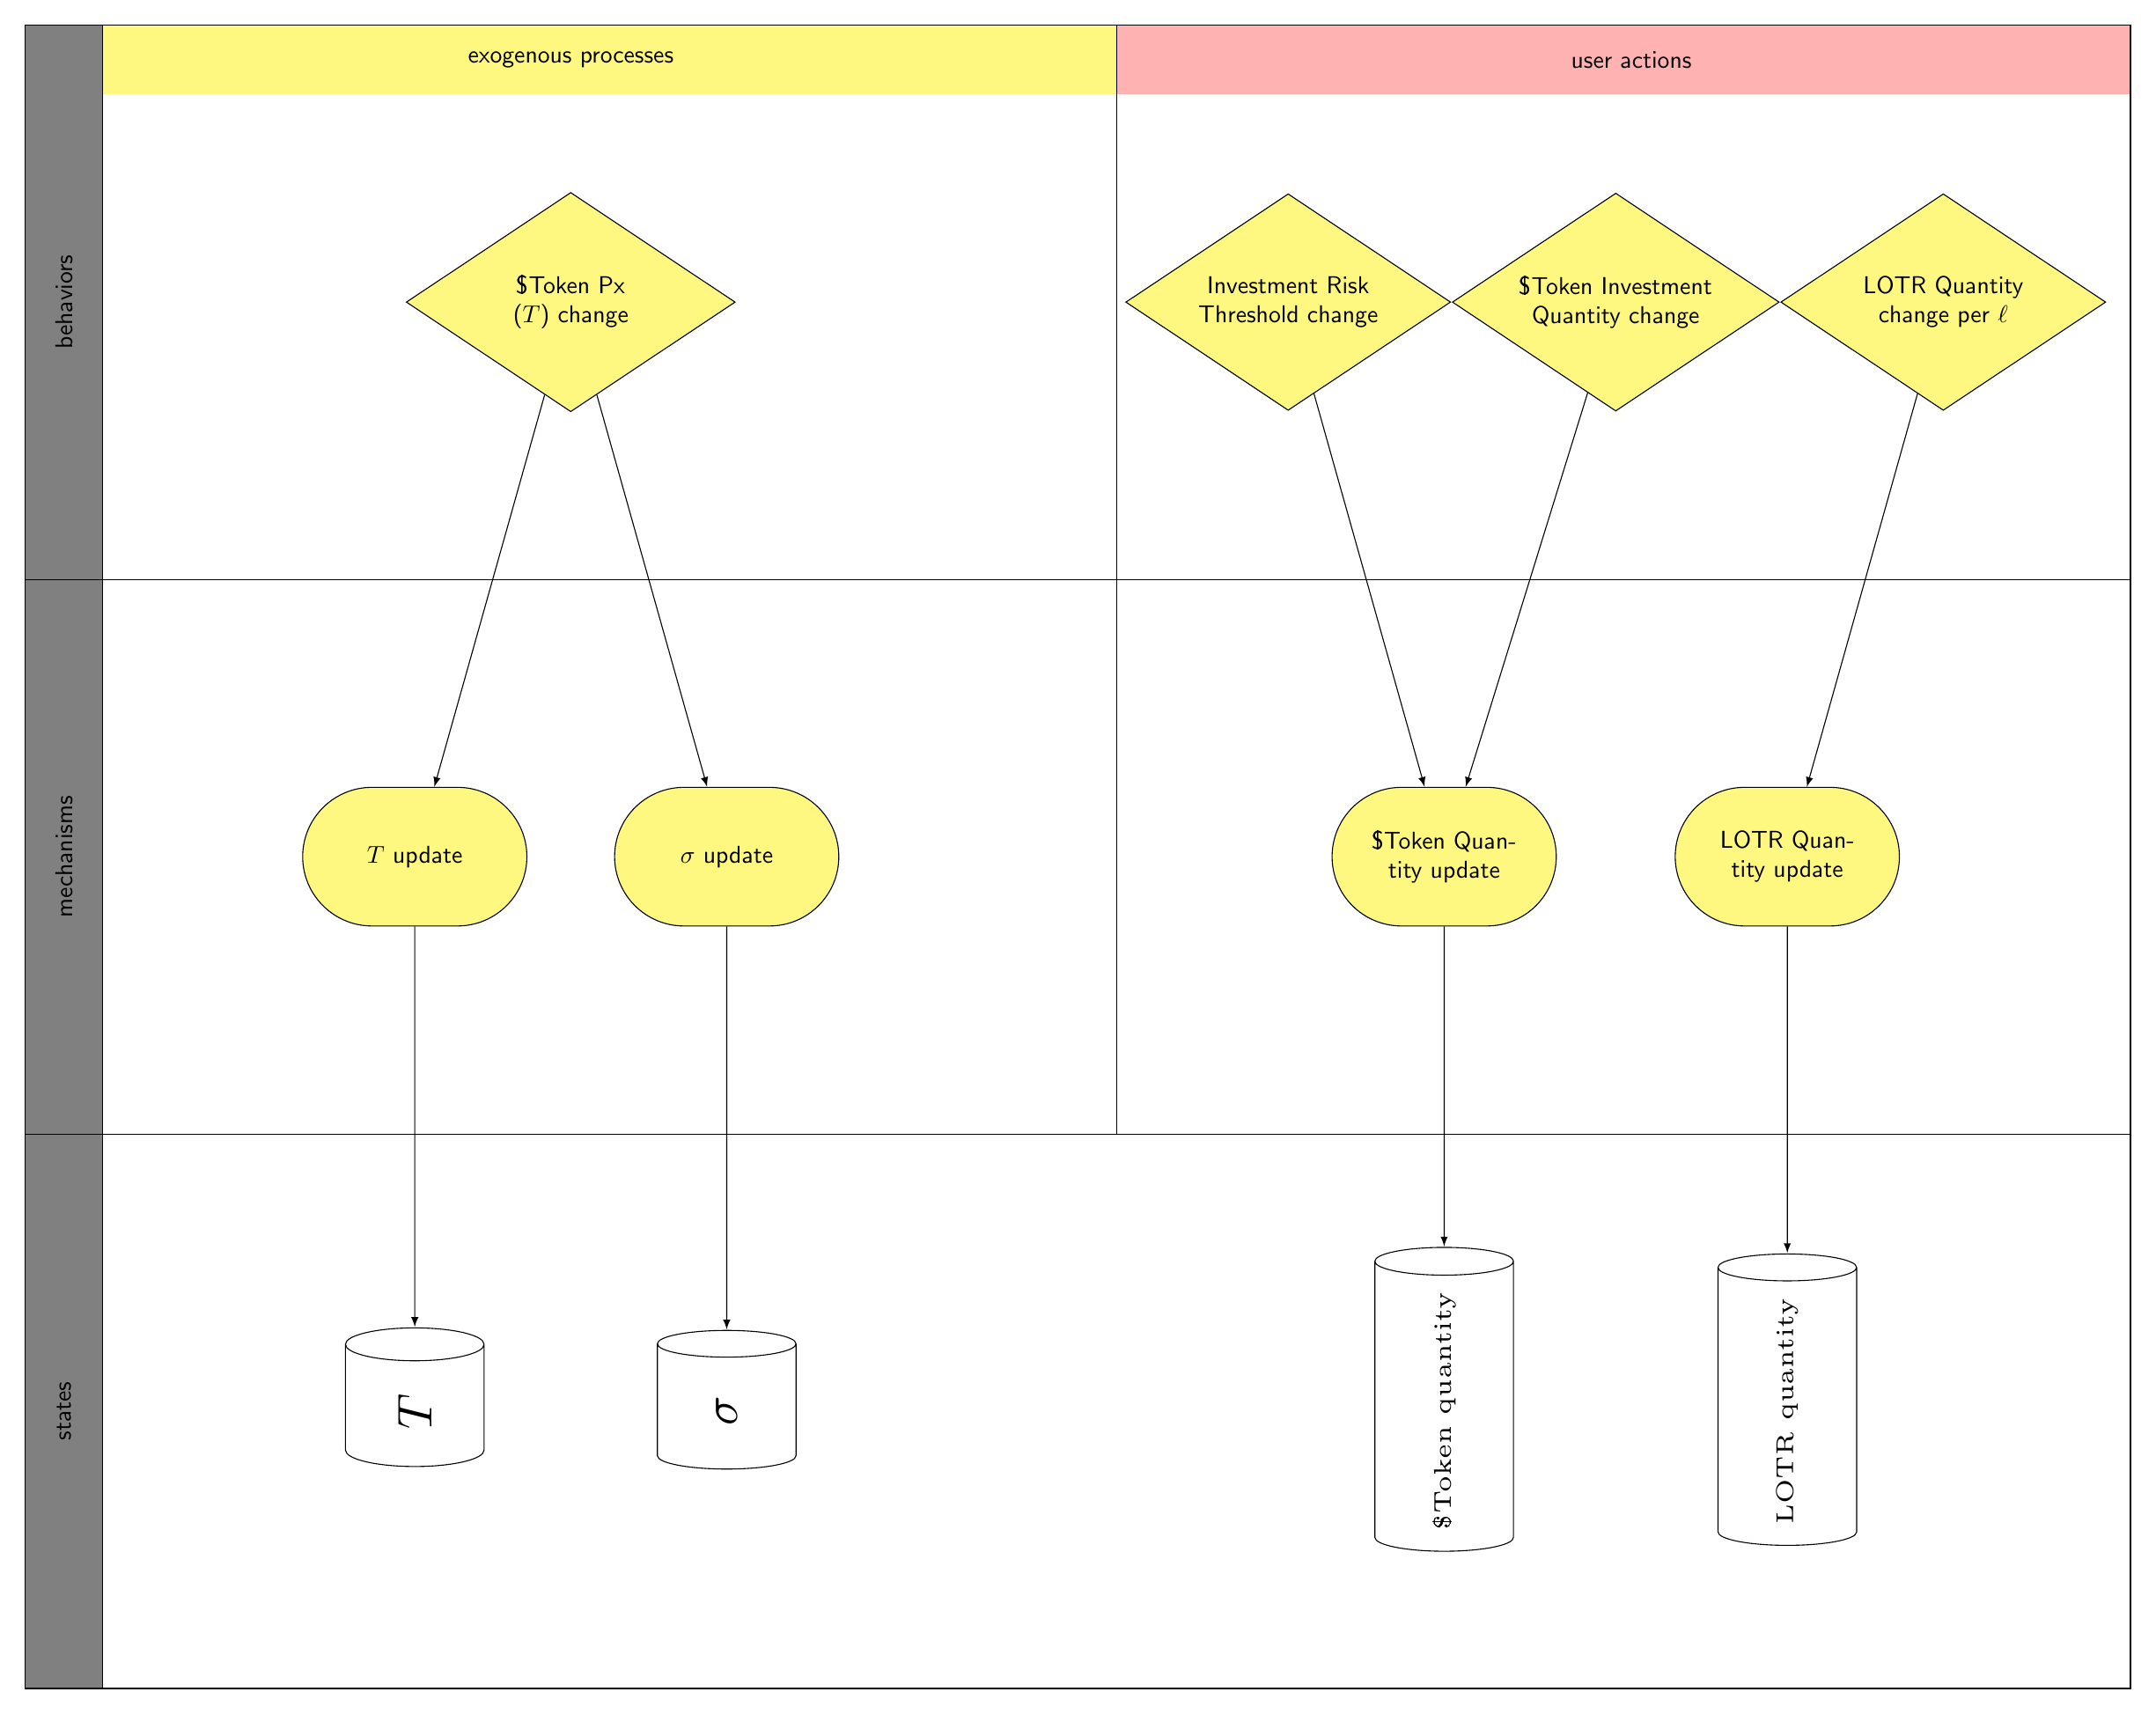
\begin{tikzpicture}[x=4.5cm,y=2cm]
        %---
        \foreach \i in {-4,0,4} {
            \fill[color=gray] (-.75,\i) rectangle (-.5,\i+4);
            \draw (-.75,\i) rectangle (6,\i+4);
        }
        \draw (-.75,-4) rectangle (-.5,0);
        \node[rotate=90,font=\sffamily] at (-.625,6) {behaviors};
        \node[rotate=90,font=\sffamily] at (-.625,2) {mechanisms};
        \node[rotate=90,font=\sffamily] at (-.625,-2) {states};

        \fill[color=yellow!50] (-.5,8) rectangle (2.75,7.5);
        \draw (-.5,8) rectangle (2.75,0);
        \fill[color=red!30] (2.75,8) rectangle (6,7.5);
        \draw (2.75,8) rectangle (6,0);
        \node[rotate=0,font=\sffamily] at (1,7.75) {exogenous processes};
        \node[rotate=0,font=\sffamily] at (4.4,7.75) {user actions};
        
        %---
        % \node[recyel] (sale1) at (0,1) {Order completed};
        \node[diayel] (b-e-t-px) at (1,6) {\$Token Px ($T$) change};
        \node[rndyel] (m-e-t-px) at (.5,2) {$T$ update};
        \node[cylwht] (s-t-px) at (.5,-2) {$T$};
        \node[cylwht] (s-t-s) at (1.5,-2) {$\sigma$};

        \node[diayel] (b-u-t-px) at (3.3,6) {Investment Risk Threshold change};
        \node[diayel] (b-u-t-q) at (4.35,6) {\$Token Investment Quantity change};
        \node[diayel] (b-u-lotr-q) at (5.4,6) {LOTR Quantity change per $\ell$};
        \node[rndyel] (m-u-t-q) at (3.8,2) {\$Token Quantity update};
        \node[rndyel] (m-u-lotr-q) at (4.9,2) {LOTR Quantity update};
        \node[cylwht] (s-t-q) at (3.8,-2) {\tiny \$Token quantity};
        \node[cylwht] (s-lotr-q) at (4.9,-2) {\tiny LOTR quantity};

        \node[rndyel] (m-e-t-s) at (1.5,2) {$\sigma$ update};

        \begin{scope}[every path/.style={-latex}]
            \draw (b-e-t-px) edge (m-e-t-px)
                (m-e-t-px) edge (s-t-px);
            \draw (b-e-t-px) edge (m-e-t-s)
                (m-e-t-s) edge (s-t-s);
            \draw (b-u-t-px) edge (m-u-t-q)
                (m-u-t-q) edge (s-t-q);
            \draw (b-u-t-q) edge (m-u-t-q);
            \draw (b-u-lotr-q) edge (m-u-lotr-q)
                (m-u-lotr-q) edge (s-lotr-q);
            % \draw (cre3) edge node[midway,fill=white,inner sep=2pt] {No} (sale3)
            % \draw (cre5.north east) -- ++(0,3);
        \end{scope}
    \end{tikzpicture}
\end{document}